\chapter{A brief taxonomy of streaming models}
\label{taxonomy}

We start by looking at how to write queries as \emph{streaming programs}, so that we may query large datasets without running out of memory.
Streaming programs consume data from their input streams element by element, processing the elements in sequential order, and need only store a limited number of elements at a time as local state.
A streaming program cannot rewind an input stream to re-read previous elements, or perform random access to read from an arbitrary element in the stream.
These restrictions mean that a streaming program cannot, for example, sort all the input data in a single pass over the input stream, because single-pass sorting requires storing all the elements in memory.
The upside of these restrictions is that if we can write our queries as streaming programs, we can be confident that they will run in constant space --- no matter how large the input stream is.
In general, input streams may be infinite, though in this thesis we focus on large but finite streams.

% With just this definition one could go and write a streaming program in more or less any language with input-output facilities.
% This is how a C programmer may implement a streaming program.
% Take, for example, the standard unix tool \Hs/wc/.
% Conceptually, this program does four things: it reads a file, counts the lines, counts the words, and counts the characters.
% One might expect these four distinct concepts to be clearly distinct in the code, but because
% Writing streaming programs in this manner can be error-prone and tedious however, as all aspects of the program must be interspersed.

Streaming, as described above, is a rather general concept.
This definition tells us what a streaming program is, but it does not offer any guidance on how to write streaming programs.
In fact, there are many ways to write streaming programs; in this thesis we restrict our attention to streaming programs written in a \emph{functional style}.
The functional style of writing streaming programs involves using small stream transformers that are composed to create larger programs.
The benefit of this style is that each stream transformer can be reasoned about and tested in isolation, without having to worry about any hidden dependencies or interference between different transformers.

There are numerous \emph{streaming models} to choose from, and we must commit to a particular model before we can start writing programs.
Choosing a streaming model requires making a trade-off between the performance overhead, which operations are supported, and the amount of extra bookkeeping the programmer must perform to write their program compared to a non-streaming implementation.
% The streaming model determines which stream operations are supported including how streams can be connected together, and the overhead incurred when connecting streams together.
% \ED{A pedantic note on terminology: the distinction between \emph{model} and \emph{representation} is that the model includes information about how the overhead is removed.}
We must compare different streaming models to make an informed decision.
We start our initial comparison by focussing on two low-overhead streaming models to illustrate how they support different operations, and to motivate the use of Kahn process networks as a streaming model.
In \cref{s:Benchmarks}, we will compare with some more expressive but less efficient streaming models.

\section{Gold panning}
\label{taxonomy/gold-panning}
% Even with the bounded memory and sequential access restrictions of streaming, we can still write interesting queries as streaming programs.
Let us now describe a situation in which we would like to execute many queries over the same dataset.
To avoid mixing up the details of streaming with the details of the example, we initially assume that the dataset fits in memory as a list, and write our queries as list programs.
Throughout the thesis, we will refer back to this example as \emph{gold panning}.

Suppose we have a file containing the historical prices for a particular corporate stock.
The file contains many records; each record contains a date and the average price for that day, and all the records in the file are sorted chronologically.
The records are stored on-disk in comma-separated values (CSV) format, and are represented in memory by the following Haskell datatype:

\begin{haskell}
data Record = Record
 { time  :: Time
 , price :: Double }
\end{haskell}

We wish to appraise this stock to see whether it was, historically, a worthy investment.
One quality of a good investment is that its price increases over time; we can quantify any increase by computing the linear regression of the price over time, using the coefficient of the line to approximate increase or decrease over time.
It is very convenient to be able to summarise growth with one number, but stock prices rarely act as lines.
While a line might be a good approximation for a stable stock price with few dips and bumps, it is a poor approximation for an unstable stock.
Fortunately, we can use a statistical tool called the \emph{Pearson correlation coefficient} to determine how linear the relationship is, and therefore how good the approximation is --- which may be valuable information about the stock price in itself as well as denoting the confidence of our analyses.
The Pearson correlation coefficient is defined as the covariance of price with time, divided by the product of the standard deviation of price and the standard deviation of time.
We can also define the Pearson correlation coefficient geometrically: it is the cosine of the angle between the regression line of price over time, and the regression line of time over price.

\newcommand\FigsStockAxisShared {width=7cm,height=7cm,}
\newcommand\FigsStockAxisTime {xlabel=Time (days),ylabel=Unit price,} % ,x tick label style={color=white},}
\newcommand\FigsStockAxisMarket {xlabel=Market percentage of mean market price,ylabel=Stock percentage of mean,}

\begin{figure}[h]
  \centering
  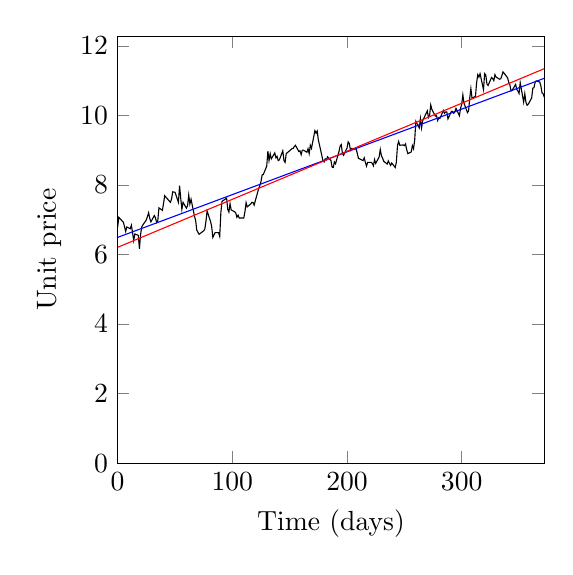
\begin{tikzpicture}
\begin{axis}[
xmin=0.0,ymin=0.0,xmax=372.0,ymax=12.268,
\FigsStockAxisShared\FigsStockAxisTime]
\addplot[
] coordinates {
(0.0,6.78)(1.0,7.07)(4.0,6.96)(5.0,6.93)(6.0,6.8)(7.0,6.66)(8.0,6.79)(11.0,6.74)(12.0,6.84)(13.0,6.63)(14.0,6.4)(15.0,6.59)(18.0,6.55)(19.0,6.16)(20.0,6.57)(21.0,6.79)(22.0,6.85)(25.0,6.99)(26.0,7.09)(27.0,7.2)(28.0,7.04)(29.0,6.94)(32.0,7.12)(33.0,7.05)(34.0,6.92)(35.0,6.97)(36.0,7.34)(39.0,7.27)(40.0,7.46)(41.0,7.69)(46.0,7.5)(47.0,7.59)(48.0,7.8)(50.0,7.79)(53.0,7.5)(54.0,7.98)(55.0,7.62)(56.0,7.3)(57.0,7.5)(60.0,7.33)(61.0,7.41)(62.0,7.71)(63.0,7.45)(64.0,7.59)(67.0,7.1)(68.0,6.98)(69.0,6.7)(70.0,6.64)(71.0,6.58)(75.0,6.68)(76.0,6.73)(77.0,6.95)(78.0,7.25)(81.0,6.95)(82.0,6.8)(83.0,6.49)(84.0,6.56)(85.0,6.63)(88.0,6.63)(89.0,6.52)(90.0,7.2)(91.0,7.53)(92.0,7.55)(95.0,7.62)(96.0,7.3)(97.0,7.22)(98.0,7.46)(99.0,7.28)(102.0,7.23)(103.0,7.19)(104.0,7.07)(105.0,7.13)(106.0,7.05)(109.0,7.05)(110.0,7.05)(111.0,7.23)(112.0,7.49)(113.0,7.37)(116.0,7.45)(117.0,7.5)(118.0,7.5)(119.0,7.42)(120.0,7.54)(123.0,7.9)(124.0,7.98)(125.0,8.1)(126.0,8.29)(127.0,8.3)(130.0,8.54)(131.0,8.97)(132.0,8.7)(133.0,8.9)(134.0,8.75)(137.0,8.92)(138.0,8.78)(139.0,8.82)(140.0,8.7)(141.0,8.72)(144.0,8.98)(145.0,8.7)(146.0,8.65)(147.0,8.9)(152.0,9.04)(153.0,9.05)(154.0,9.1)(155.0,9.14)(158.0,8.96)(159.0,8.98)(160.0,8.87)(161.0,9.0)(162.0,9.0)(165.0,8.94)(166.0,9.04)(167.0,8.9)(168.0,9.14)(169.0,9.05)(172.0,9.56)(173.0,9.49)(174.0,9.55)(175.0,9.29)(176.0,9.15)(179.0,8.7)(180.0,8.66)(181.0,8.75)(182.0,8.72)(183.0,8.81)(186.0,8.7)(187.0,8.51)(188.0,8.5)(189.0,8.66)(190.0,8.61)(193.0,8.96)(194.0,9.12)(195.0,9.16)(196.0,8.9)(197.0,8.85)(200.0,9.06)(201.0,9.24)(202.0,9.19)(203.0,9.0)(204.0,9.05)(208.0,9.03)(209.0,8.9)(210.0,8.76)(211.0,8.75)(214.0,8.7)(215.0,8.78)(216.0,8.65)(217.0,8.54)(218.0,8.65)(221.0,8.65)(222.0,8.62)(223.0,8.55)(224.0,8.73)(225.0,8.62)(228.0,8.8)(229.0,9.02)(230.0,8.84)(231.0,8.77)(232.0,8.68)(235.0,8.6)(236.0,8.69)(237.0,8.62)(238.0,8.56)(239.0,8.63)(242.0,8.5)(243.0,8.65)(244.0,9.13)(245.0,9.25)(246.0,9.14)(249.0,9.15)(250.0,9.13)(251.0,9.18)(252.0,9.02)(253.0,8.9)(256.0,8.95)(257.0,9.13)(258.0,9.04)(259.0,9.29)(260.0,9.83)(263.0,9.64)(264.0,9.91)(265.0,9.64)(266.0,9.85)(267.0,9.92)(270.0,10.13)(271.0,9.94)(272.0,10.0)(273.0,10.3)(274.0,10.17)(277.0,9.98)(278.0,10.0)(279.0,9.85)(280.0,9.92)(281.0,9.91)(284.0,10.14)(285.0,10.06)(286.0,10.1)(287.0,10.1)(288.0,9.9)(291.0,10.11)(292.0,10.11)(293.0,10.06)(294.0,10.1)(295.0,10.2)(298.0,9.99)(299.0,10.2)(300.0,10.32)(301.0,10.59)(302.0,10.35)(305.0,10.08)(306.0,10.13)(307.0,10.5)(308.0,10.77)(309.0,10.49)(312.0,10.55)(313.0,10.94)(314.0,11.17)(315.0,11.1)(316.0,11.2)(319.0,10.74)(320.0,11.2)(321.0,11.16)(322.0,10.9)(323.0,10.86)(326.0,11.09)(327.0,11.06)(328.0,11.0)(329.0,11.17)(330.0,11.1)(333.0,11.04)(334.0,11.05)(335.0,11.14)(336.0,11.25)(337.0,11.21)(340.0,11.08)(341.0,10.95)(342.0,10.88)(343.0,10.7)(344.0,10.72)(347.0,10.89)(348.0,10.75)(349.0,10.7)(350.0,10.63)(351.0,10.94)(354.0,10.38)(355.0,10.62)(356.0,10.38)(357.0,10.29)(358.0,10.32)(361.0,10.5)(362.0,10.78)(363.0,10.8)(364.0,10.95)(365.0,10.99)(368.0,10.96)(369.0,10.85)(370.0,10.65)(371.0,10.62)(372.0,10.52)
};
% Correlation: 0.9435949591611904
\addplot [blue,domain=0.0:372.0] { 6.491020041524747 + 1.2297326026911954e-2 * x };
\addplot [red,domain=0.0:372.0] { 6.20504166235812 + 1.381145595916851e-2 * x };
\end{axis}
\end{tikzpicture}

  \caption{Analysis of a stock over a year}
  \label{fig:stock:it:stock-over-time}
\end{figure}


\Cref{fig:stock:it:stock-over-time} shows the fluctuations of the example stock's price over a year, along with the regression line of price over time in red, and the regression line of time over price in blue.
The stock price is far from a perfect line, but does show a clear upwards trend.
% The correlation coefficient is a scalar ranging from negative one to positive one.
In this graph, the correlation is represented by the angle between the red and blue regression lines; the smaller the angle between the two regression lines, the more closely correlated the two are, and the `straighter' the relationship is.
The angle here corresponds to a correlation of $0.94$, in a range from negative one to positive one.

% We can roughly quantify whether or not price increases over time by computing the Pearson correlation coefficient of the two.
% The Pearson correlation coefficient represents how well the relationship can be approximated by a linear function and ranges from negative one to one; a correlation of one denotes that price grows linearly with time, while a correlation of negative one denotes that price decreases linearly with time.
% When the relationship is non-linear but does still tend to increase over time, the correlation will be a positive number between zero and one.

\begin{haskell}[float,label=figs/impl/correlation-multi,caption=Multiple-pass correlation implementation]
correlation :: [(Double,Double)] -> Double
correlation xys = covariance xys / stddev (map fst xys) * stddev (map snd xys)

stddev :: [Double] -> Double
stddev xs = sqrt (mean (map (^2) xs) / mean xs * mean xs)

covariance :: [(Double,Double)] -> Double
covariance xys =
 let xy = map (\(x,y) -> x * y) xys
 in mean xy - mean (map fst xys) * mean (map snd xys)

mean :: [Double] -> Double
mean xs = sum xs / fromIntegral (length xs)
\end{haskell}

\begin{haskell}[float,label=figs/impl/correlation,caption=One-pass correlation implementation]
type State = (Double, Double, Double, Double, Double, Double)
correlation_z :: State
correlation_z = (0,0,0,0,0,0)

correlation_k :: State -> (Double,Double) -> State
correlation_k (mx, my, sd, sdX, sdY, n) (x,y) =
 let n'   = n   + 1
     dx   = x   - mx
     dy   = y   - my
     mx'  = mx  + (dx / n')
     my'  = my  + (dy / n')
     dx'  = x   - my'
     dy'  = y   - my'
     sd'  = sd  + dx * dy'
     sdX' = sdX + dx * dx'
     sdY' = sdY + dy * dy'
 in (mx',my',sd',sdX',sdY',n')

correlation_x :: State -> Double
correlation_x (mx, my, sd, sdX, sdY, n) =
  let varianceX  = sdX / n
      varianceY  = sdY / n
      covariance = sd  / n
      stddevX = sqrt varianceX
      stddevY = sqrt varianceY
  in covariance / (stddevX * stddevY)
\end{haskell}


\cref{figs/impl/correlation-multi} contains the implementations of functions to compute the correlation coefficient, directly translated from the mathematical definitions.
This implementation performs multiple passes over the input list, and is not numerically stable.

We can implement a more stable one-pass correlation algorithm using the covariance algorithm specified in \citet{welford1962note}.
Although the details are quite complicated, we can express this algorithm as a fold over a list.
The fold uses an initial state, \Hs/correlation_z/, and for each element updates the state with a worker function \Hs/correlation_k/.
The one-pass correlation algorithm keeps track of the running means and standard deviations of both axes, which are used to compute the correlation.
As such, the fold state contains more than just the correlation.
After the fold has completed, we perform an \emph{extraction} function, \Hs/correlation_x/, to extract the correlation from the state.
\Cref{figs/impl/correlation} contains the implementations of the fold worker functions for computing the correlation: \Hs/correlation_x/, \Hs/correlation_k/ and \Hs/correlation_z/.
With these worker functions, we can compute the correlation as follows:

\begin{haskell}
correlation :: [(Double,Double)] -> Double
correlation = correlation_x (foldl correlation_k correlation_z)
\end{haskell}


We can implement a function to compute the regression similarly; we omit the definitions of the regression worker functions.
The definition of the function to compute the regression uses the fold worker functions \Hs/regression_x/ for extracting the final result, \Hs/regression_z/ for the initial state, and \Hs/regression_k/ to update the state for every input element:

\begin{haskell}
regression :: [(Double,Double)] -> Line
regression = regression_x (foldl regression_k regression_z)
\end{haskell}

Now that we have functions to compute the linear regression and the correlation, we can compute both at the same time.
The following program returns a pair containing the correlation and regression:

\begin{haskell}
priceOverTime :: [Record] -> (Line, Double)
priceOverTime stock =
  let timeprices = map (\r -> (daysSinceEpoch (time r), price r)) stock
  in (regression timeprices, correlation timeprices)
\end{haskell}

Both \Hs/regression/ and \Hs/correlation/ functions take a list of pairs of numbers, so we first convert the \Hs/Record/ values to pairs of numbers using the \Hs/map/ combinator.
Although this is a single program, it computes two values.
Whether we think of this program as one query or two is inconsequential.
The important part is that this program, as it is written, requires two traversals over the \Hs/timeprices/ list.
List programs can traverse the same list many times; in \cref{taxonomy/pull} we shall see how multiple traversals is a problem for streaming programs.

Stock prices rarely follow linear functions of time; even the best stocks go down once in a while, and sometimes the market as a whole can go down.
Furthermore, even though this stock appears to be doing quite well if we consider it in isolation, we do not know whether it is an exceptional stock or an exceptional market.
We are interested in comparing against the rest of the market as well.

To compare against the rest of the market, we have another file of records containing the average price of a representative subset of stocks.
This representative subset is called a \emph{market index}.
We want to compare each day's price for our stock against the average price for the corresponding day in the index.

\begin{figure}[h]
  \centering
  \begin{subfigure}[t]{0.45\textwidth}
    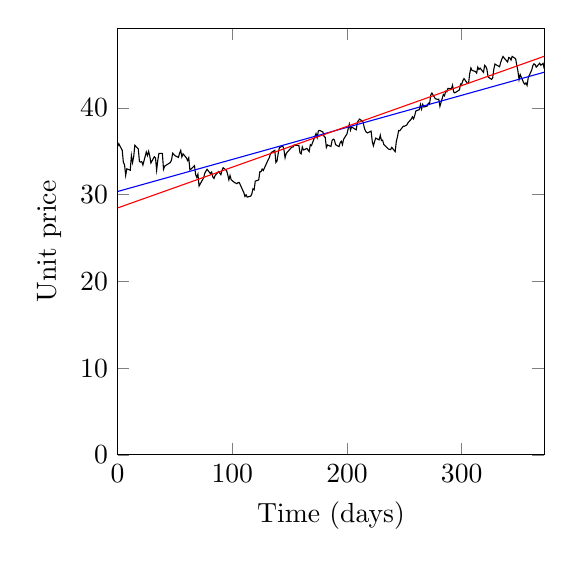
\begin{tikzpicture}
\begin{axis}[
xmin=0.0,ymin=0.0,xmax=372.0,ymax=49.174,
\FigsStockAxisShared\FigsStockAxisTime]
\addplot[
] coordinates {
(0.0,35.54)(1.0,35.86)(4.0,35.1)(5.0,33.7)(6.0,33.46)(7.0,32.22)(8.0,32.97)(11.0,32.81)(12.0,34.49)(13.0,33.7)(14.0,34.38)(15.0,35.68)(18.0,35.26)(19.0,33.8)(20.0,33.75)(21.0,33.8)(22.0,33.4)(25.0,34.91)(26.0,34.5)(27.0,34.98)(28.0,34.46)(29.0,33.64)(32.0,34.37)(33.0,34.24)(34.0,32.82)(35.0,33.95)(36.0,34.75)(39.0,34.75)(40.0,32.92)(41.0,33.28)(46.0,33.7)(47.0,34.0)(48.0,34.77)(50.0,34.49)(53.0,34.28)(54.0,34.77)(55.0,35.1)(56.0,34.34)(57.0,34.7)(60.0,34.22)(61.0,33.92)(62.0,34.24)(63.0,32.85)(64.0,32.94)(67.0,33.33)(68.0,32.31)(69.0,31.99)(70.0,32.35)(71.0,30.99)(75.0,31.94)(76.0,32.46)(77.0,32.71)(78.0,32.91)(81.0,32.4)(82.0,32.6)(83.0,32.02)(84.0,31.86)(85.0,32.2)(88.0,32.65)(89.0,32.48)(90.0,32.3)(91.0,32.77)(92.0,33.1)(95.0,32.77)(96.0,32.29)(97.0,31.7)(98.0,32.2)(99.0,31.71)(102.0,31.38)(103.0,31.33)(104.0,31.25)(105.0,31.37)(106.0,31.4)(109.0,30.52)(110.0,30.23)(111.0,29.79)(112.0,29.97)(113.0,29.71)(116.0,29.82)(117.0,30.07)(118.0,30.67)(119.0,30.55)(120.0,31.55)(123.0,31.69)(124.0,32.63)(125.0,32.64)(126.0,32.94)(127.0,32.78)(130.0,33.65)(131.0,33.95)(132.0,34.19)(133.0,34.6)(134.0,34.85)(137.0,35.1)(138.0,33.71)(139.0,33.88)(140.0,34.74)(141.0,35.41)(144.0,35.62)(145.0,35.16)(146.0,34.24)(147.0,34.75)(152.0,35.5)(153.0,35.48)(154.0,35.72)(155.0,35.68)(158.0,35.67)(159.0,34.8)(160.0,34.69)(161.0,35.48)(162.0,35.14)(165.0,35.32)(166.0,35.12)(167.0,34.96)(168.0,35.75)(169.0,35.65)(172.0,36.7)(173.0,37.03)(174.0,36.57)(175.0,37.32)(176.0,37.4)(179.0,37.21)(180.0,36.71)(181.0,36.59)(182.0,35.43)(183.0,35.72)(186.0,35.55)(187.0,36.26)(188.0,36.39)(189.0,36.29)(190.0,35.75)(193.0,35.53)(194.0,35.96)(195.0,36.15)(196.0,35.75)(197.0,36.37)(200.0,37.01)(201.0,37.59)(202.0,38.11)(203.0,37.42)(204.0,37.8)(208.0,37.46)(209.0,38.29)(210.0,38.55)(211.0,38.7)(214.0,38.38)(215.0,37.73)(216.0,37.35)(217.0,37.17)(218.0,37.11)(221.0,37.31)(222.0,36.13)(223.0,35.62)(224.0,36.1)(225.0,36.51)(228.0,36.3)(229.0,36.85)(230.0,36.23)(231.0,36.28)(232.0,35.8)(235.0,35.4)(236.0,35.26)(237.0,35.21)(238.0,35.18)(239.0,35.44)(242.0,34.95)(243.0,36.13)(244.0,36.67)(245.0,37.38)(246.0,37.36)(249.0,37.87)(250.0,37.88)(251.0,37.95)(252.0,38.0)(253.0,38.25)(256.0,38.7)(257.0,38.97)(258.0,38.73)(259.0,39.1)(260.0,39.64)(263.0,39.79)(264.0,40.4)(265.0,39.86)(266.0,40.4)(267.0,40.09)(270.0,40.22)(271.0,40.54)(272.0,40.48)(273.0,41.46)(274.0,41.71)(277.0,41.04)(278.0,41.01)(279.0,40.97)(280.0,40.99)(281.0,40.18)(284.0,41.54)(285.0,41.39)(286.0,41.92)(287.0,41.84)(288.0,42.24)(291.0,42.2)(292.0,42.61)(293.0,41.82)(294.0,41.73)(295.0,41.81)(298.0,42.06)(299.0,42.75)(300.0,42.72)(301.0,43.15)(302.0,43.37)(305.0,42.81)(306.0,42.87)(307.0,43.96)(308.0,44.59)(309.0,44.32)(312.0,44.18)(313.0,44.0)(314.0,44.68)(315.0,44.43)(316.0,44.58)(319.0,44.09)(320.0,44.89)(321.0,44.76)(322.0,44.43)(323.0,43.55)(326.0,43.28)(327.0,43.45)(328.0,44.46)(329.0,45.05)(330.0,44.96)(333.0,44.74)(334.0,45.24)(335.0,45.62)(336.0,45.92)(337.0,45.74)(340.0,45.28)(341.0,45.8)(342.0,45.74)(343.0,45.51)(344.0,45.93)(347.0,45.66)(348.0,44.92)(349.0,44.25)(350.0,43.25)(351.0,43.84)(354.0,42.89)(355.0,42.72)(356.0,42.86)(357.0,42.58)(358.0,43.48)(361.0,44.35)(362.0,44.87)(363.0,45.07)(364.0,44.98)(365.0,44.69)(368.0,45.14)(369.0,44.91)(370.0,45.02)(371.0,45.12)(372.0,44.49)
};
% Correlation: 0.8868243284601378
\addplot [blue,domain=0.0:372.0] { 30.357224182011205 + 3.695729147936317e-2 * x };
\addplot [red,domain=0.0:372.0] { 28.461917295110723 + 4.699210913456761e-2 * x };
\end{axis}
\end{tikzpicture}

    \caption{Market over time}
    \label{fig:stock:it:market-over-time}
  \end{subfigure}
  \quad
  \begin{subfigure}[t]{0.45\textwidth}
    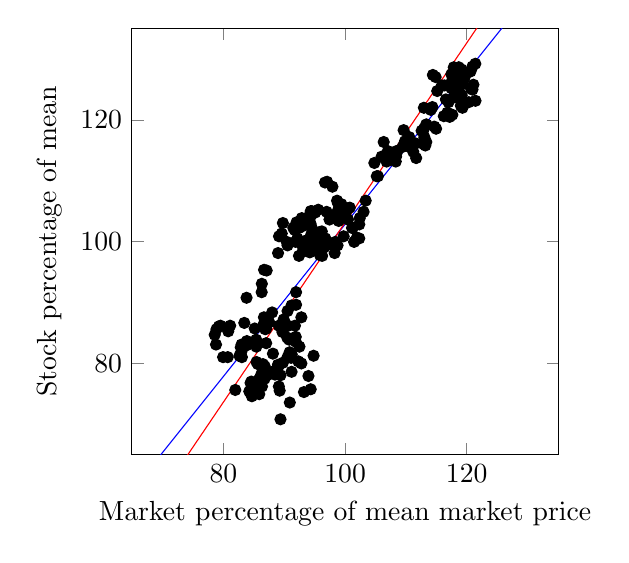
\begin{tikzpicture}
\begin{axis}[
xmin=64.91671453187823,ymin=64.91671453187823,xmax=135.08328546812177,ymax=135.08328546812177,
\FigsStockAxisShared\FigsStockAxisMarket]
\addplot[
only marks] coordinates {
(93.97144368059229,77.88627225732337)(94.81755684822845,81.21769098219414)(92.80803807509255,79.95404939689833)(89.1062929666843,79.60941987363583)(88.47170809095716,78.1160252728317)(85.193019566367,76.50775416427341)(87.17609730301427,78.00114876507755)(86.75304071919619,77.42676622630673)(91.19513484928609,78.57553130384835)(89.1062929666843,76.16312464101091)(90.90428344791115,73.52096496266513)(94.34161819143311,75.70361860999425)(93.23109465891062,75.24411257897759)(89.3707033315706,70.7639287765652)(89.23849814912744,75.47386559448593)(89.3707033315706,78.00114876507755)(88.31306187202537,78.69040781160253)(92.30565838180856,80.29867892016082)(91.22157588577473,81.44744399770246)(92.49074563722897,82.71108558299828)(91.1158117398202,80.87306145893164)(88.94764674775251,79.72429638139002)(90.87784241142252,81.79207352096496)(90.53410893707033,80.9879379666858)(86.77948175568481,79.49454336588168)(89.76731887890006,80.0689259046525)(91.88260179799047,84.31935669155658)(91.88260179799047,83.51522113727742)(87.04389212057113,85.69787478460654)(87.99576943416182,88.34003446295233)(89.1062929666843,86.15738081562321)(89.8995240613432,87.19126938541069)(91.93548387096774,89.60367604824813)(91.19513484928609,89.48879954049397)(90.63987308302485,86.15738081562321)(91.93548387096774,91.67145318782309)(92.80803807509255,87.53589890867318)(90.79851930195665,83.85985066053992)(91.75039661554733,86.15738081562321)(90.48122686409307,84.20448018380242)(89.68799576943417,85.12349224583573)(90.53410893707033,88.56978747846065)(86.85880486515072,85.58299827685238)(87.09677419354837,87.19126938541069)(88.12797461660496,81.56232050545663)(85.43098889476468,80.18380241240666)(84.58487572712849,76.96726019529007)(85.5367530407192,76.27800114876507)(81.94077207826547,75.58874210224009)(84.45267054468536,76.73750717978173)(85.82760444209413,77.31188971855256)(86.48863035430989,79.83917288914417)(87.01745108408248,83.2854681217691)(85.66895822316233,79.83917288914417)(86.19777895293495,78.1160252728317)(84.66419883659441,74.55485353245261)(84.2411422527763,75.35898908673175)(85.14013749338974,76.16312464101091)(86.3299841353781,76.16312464101091)(85.88048651507138,74.8994830557151)(85.40454785827603,82.71108558299828)(86.64727657324168,86.50201033888571)(87.51983077736648,86.73176335439402)(86.64727657324168,87.53589890867318)(85.37810682178741,83.85985066053992)(83.81808566895822,82.9408385985066)(85.14013749338974,85.69787478460654)(83.84452670544685,83.6300976450316)(82.97197250132204,83.05571510626078)(82.8397673188789,82.59620907524412)(82.62823902696985,81.21769098219414)(82.94553146483342,81.90695002871912)(83.02485457429931,80.9879379666858)(80.69804336329985,80.9879379666858)(79.93125330512956,80.9879379666858)(78.76784769962983,83.05571510626078)(79.24378635642518,86.04250430786904)(78.55631940772079,84.66398621481906)(78.84717080909572,85.58299827685238)(79.50819672131148,86.15738081562321)(81.0946589106293,86.15738081562321)(80.77736647276573,85.23836875358988)(83.42147012162877,86.61688684663986)(83.7916446324696,90.75244112578979)(86.27710206240086,91.67145318782309)(86.30354309888948,93.04997128087305)(87.09677419354837,95.23262492820217)(86.6737176097303,95.34750143595635)(88.97408778424114,98.10453762205627)(89.76731887890006,103.04422745548536)(90.40190375462717,99.9425617461229)(91.48598625066103,102.2400919012062)(92.14701216287679,100.51694428489373)(92.80803807509255,102.46984491671454)(89.13273400317293,100.86157380815621)(89.58223162347964,101.3210798391729)(91.85616076150185,99.9425617461229)(93.62771020624008,100.17231476163124)(94.18297197250132,103.15910396323953)(92.96668429402432,99.9425617461229)(90.53410893707033,99.3681792073521)(91.88260179799047,102.2400919012062)(93.86567953463776,103.8483630097645)(93.8127974616605,103.96323951751867)(94.44738233738762,104.53762205628949)(94.34161819143311,104.99712808730615)(94.31517715494448,102.9293509477312)(92.01480698043363,103.15910396323953)(91.7239555790587,101.89546237794369)(93.8127974616605,103.38885697874784)(92.91380222104706,103.38885697874784)(93.38974087784241,102.69959793222286)(92.8609201480698,103.8483630097645)(92.43786356425173,102.2400919012062)(94.52670544685353,104.99712808730615)(94.26229508196721,103.96323951751867)(97.0386039132734,109.82194141298105)(97.9111581173982,109.01780585870189)(96.69487043892121,109.70706490522689)(98.67794817556849,106.7202757036186)(98.88947646747752,105.11200459506031)(98.38709677419355,99.9425617461229)(97.06504494976204,99.48305571510626)(96.74775251189848,100.51694428489373)(93.68059227921735,100.17231476163124)(94.44738233738762,101.20620333141872)(93.99788471708091,99.9425617461229)(95.87519830777366,97.75990809879379)(96.21893178212586,97.64503159103964)(95.95452141723956,99.48305571510626)(94.52670544685353,98.90867317633543)(93.94500264410365,102.9293509477312)(95.08196721311477,104.7673750717978)(95.58434690639874,105.22688110281449)(94.52670544685353,102.2400919012062)(96.1660497091486,101.66570936243538)(97.85827604442093,104.07811602527283)(99.3918561607615,106.14589316484779)(100.76679005817029,105.57151062607697)(98.94235854045479,103.38885697874784)(99.94711792702273,103.96323951751867)(99.04812268640931,103.73348650201034)(101.24272871496562,102.2400919012062)(101.93019566367,100.6318207926479)(102.32681121099947,100.51694428489373)(101.4806980433633,99.9425617461229)(99.76203067160232,100.86157380815621)(98.75727128503438,99.3681792073521)(98.28133262823903,98.10453762205627)(98.12268640930725,99.3681792073521)(98.65150713907985,99.3681792073521)(95.53146483342148,99.0235496840896)(94.18297197250132,98.21941412981046)(95.45214172395559,100.28719126938542)(96.53622421998942,99.0235496840896)(95.98096245372818,101.09132682366457)(97.43521946060287,103.61860999425616)(95.79587519830777,101.5508328546812)(95.92808038075093,100.74669730040206)(94.65891062929666,99.71280873061458)(93.60126916975145,98.79379666858127)(93.23109465891062,99.82768523836874)(93.09888947646748,99.0235496840896)(93.01956636700159,98.33429063756462)(93.70703331570597,99.13842619184378)(92.4114225277631,97.64503159103964)(95.53146483342148,99.3681792073521)(96.95928080380752,104.882251579552)(98.83659439450027,106.26076967260197)(98.783712321523,104.99712808730615)(100.13220518244314,105.11200459506031)(100.15864621893178,104.882251579552)(100.34373347435219,105.4566341183228)(100.47593865679534,103.61860999425616)(101.13696456901111,102.2400919012062)(102.32681121099947,102.81447443997702)(103.04071919619248,104.882251579552)(102.40613432046534,103.8483630097645)(103.38445267054468,106.7202757036186)(104.81226864093071,112.92360712234348)(105.20888418826017,110.74095347501436)(106.82178741406662,113.84261918437679)(105.39397144368058,110.74095347501436)(106.82178741406662,113.1533601378518)(106.00211528291909,113.95749569213096)(106.34584875727128,116.36990235496842)(107.19196192490745,114.18724870763927)(107.03331570597567,114.87650775416427)(109.62453728186145,118.32280298678921)(110.28556319407721,116.82940838598506)(108.51401374933897,114.64675473865596)(108.43469063987308,114.87650775416427)(108.32892649391856,113.1533601378518)(108.38180856689583,113.95749569213096)(106.24008461131676,113.84261918437679)(109.83606557377048,116.48477886272258)(109.43945002644104,115.56576680068926)(110.84082496033845,116.02527283170592)(110.6292966684294,116.02527283170592)(111.68693812797461,113.72774267662263)(111.5811739820201,116.14014933946007)(112.66525647805395,116.14014933946007)(110.57641459545214,115.56576680068926)(110.33844526705445,116.02527283170592)(110.54997355896352,117.17403790924755)(111.21099947117928,114.7616312464101)(113.03543098889477,117.17403790924755)(112.95610787942887,118.55255600229752)(114.09307244843998,121.65422171165996)(114.67477525118983,118.89718552556002)(113.19407720782655,115.79551981619758)(113.35272342675833,116.36990235496842)(116.23479640401904,120.62033314187248)(117.90058170280275,123.72199885123491)(117.18667371760974,120.50545663411833)(116.81649920676891,121.1947156806433)(116.34056054997355,125.6748994830557)(118.13855103120041,128.3170591614015)(117.47752511898466,127.51292360712235)(117.87414066631412,128.66168868466397)(116.57852987837126,123.37736932797243)(118.69381279746165,128.66168868466397)(118.35007932310945,128.20218265364733)(117.47752511898466,125.21539345203907)(115.15071390798519,124.7558874210224)(114.43680592279217,127.39804709936817)(114.8863035430989,127.05341757610569)(117.55684822845056,126.36415852958069)(119.11686938127974,128.3170591614015)(118.87890005288206,127.51292360712235)(118.29719725013221,126.82366456059735)(119.61924907456374,126.93854106835154)(120.62400846113167,127.97242963813899)(121.4172395557906,129.2360712234348)(120.94130089899524,128.77656519241816)(119.72501322051825,127.28317059161402)(121.09994711792702,125.78977599080987)(120.94130089899524,124.98564043653073)(120.33315705975673,122.91786329695576)(121.44368059227921,123.14761631246411)(120.72977260708619,125.1005169442849)(118.77313590692755,123.4922458357266)(117.00158646218932,122.91786329695576)(114.35748281332627,122.11372774267663)(115.91750396615548,125.6748994830557)(113.4056054997356,119.24181504882252)(112.95610787942887,121.99885123492244)(113.3262823902697,119.24181504882252)(112.58593336858804,118.20792647903502)(114.96562665256478,118.55255600229752)(117.26599682707561,120.62033314187248)(118.64093072448438,123.83687535898909)(119.16975145425701,124.06662837449743)(118.93178212585933,125.78977599080987)(118.16499206768904,126.24928202182655)(119.35483870967742,125.90465249856406)(118.74669487043892,124.64101091326822)(119.03754627181387,122.34348075818495)(119.30195663670015,121.99885123492244)(117.63617133791644,120.85008615738082)
};
% Correlation: 0.9204524313502235
\addplot [blue,domain=64.91671453187823:135.08328546812177] { -22.215696740041096 + 1.2505948527539763 * x };
\addplot [red,domain=64.91671453187823:135.08328546812177] { -44.47787554503556 + 1.4760937398536222 * x };
\end{axis}
\end{tikzpicture}

    \caption{Stock over market}
    \label{fig:stock:it:stock-over-market}
  \end{subfigure}

  \caption{Analysis of a stock compared to market index}
  \label{fig:stock:it}
\end{figure}



\Cref{fig:stock:it:market-over-time} shows the linear regression and correlation of the market index price over time, while \cref{fig:stock:it:stock-over-market} shows the linear regression and correlation of the stock price from \cref{fig:stock:it:stock-over-time} compared to the market index price.
The comparison of stock price to market index price compares each day's stock price against the corresponding day's market index price.
Each day is visualised as the percentage difference between the day's stock price and the mean stock price for the period for the y axis, compared to the percentage difference between the day's market index price and the mean market index price for the period for the x axis.
We can inspect the regression lines to see how the stock price tends to react to movement in the market index price.
Both regression lines are slightly steeper than forty-five degrees, indicating that the stock price has grown faster than the market index price.
The correlation, represented by the angle between the two regression lines, indicates a relatively strong linear relationship between the stock price and the market index price.

We can compute the comparison of stock price over market index price with the following program:

\begin{haskell}
priceOverMarket :: [Record] -> [Record] -> (Line, Double)
priceOverMarket stock index =
  let joined = join (\s i   -> compare (time s) (time i)) stock index
      prices = map  (\(s,i) -> (price s, price i))        joined
  in (regression prices, correlation prices)
\end{haskell}

The \Hs/join/ operator matches each stock day against the corresponding market index day, and discards the data for any days missing from either input.
We then extract both prices from the joined result and compute the regression and correlation.
As with \Hs/priceOverTime/, this function requires two traversals of the \Hs/prices/ list.

Since the analyses \Hs/priceOverTime/ and \Hs/priceOverMarket/ both provide useful information, we will perform both.
It is just as easy to combine these queries together as it was to compute both the correlation and the regression.
The following program computes both:

\begin{haskell}
priceAnalyses :: [Record] -> [Record] -> ((Line, Double), (Line, Double))
priceAnalyses stock index =
  let pot = priceOverTime   stock
      pom = priceOverMarket stock index
  in (pot, pom)
\end{haskell}

% \begin{figure}[h]
\center
\begin{dot2tex}[dot]
digraph G {
  node [shape="none"];
  stock [texlbl="\Hs/stock/"];
  index [texlbl="\Hs/index/"];

  stock -> pom_join;
  index -> pom_join;
  stock -> pot_tps;

  graph [style="rounded corners"];

  subgraph cluster_priceOverTime  {
    lblstyle="right";
    texlbl="\Hs/priceOverTime/";
    label="  priceOverTime";
    pot_tps [texlbl="\Hs/timeprices/"];
    pot_cor [texlbl="\Hs/correlation/"];
    pot_reg [texlbl="\Hs/regression/"];
    pot_tps -> pot_cor;
    pot_tps -> pot_reg;
  };

  subgraph cluster_priceAgainstMarket {
    lblstyle="left,xshift=0.2cm";
    texlbl="\Hs/priceOverMarket/";
    label="priceOverMarket";
    pom_join [texlbl="\Hs/joined/"];
    pom_price [texlbl="\Hs/prices/"];
    pom_cor [texlbl="\Hs/correlation/"];
    pom_reg [texlbl="\Hs/regression/"];
    pom_join -> pom_price;
    pom_price -> pom_cor;
    pom_price -> pom_reg;
  };
}
\end{dot2tex}
\caption{Dependency graph for queries \Hs/priceOverTime/ and \Hs/priceOverMarket/}
\label{figs/procs/priceOverTime-priceOverMarket}
\end{figure}



\FigurePdfLabel{figs/depgraphs/priceOverTime-priceOverMarket}{figs/procs/priceOverTime-priceOverMarket}{Dependency graph for queries \Hs/priceOverTime/ and \Hs/priceOverMarket/}

\Cref{figs/procs/priceOverTime-priceOverMarket} shows the dependency graph for both queries.
The nodes in this graph are the two input lists \Hs/stock/ and \Hs/index/, and the list operators in each query.
The two input lists are drawn inside boxes to distinguish them from the operator nodes.
% each intermediate list, and the \Hs/correlation/ and \Hs/regression/ functions which summarise the list values.
The edges are dependencies from one value to another; the \Hs/join/ operator uses both the \Hs/stock/ and \Hs/index/ lists, so there are arrows from both \Hs/stock/ and \Hs/index/ to the \Hs/join/ node.
Edges that denote intermediate lists between two operators are labelled with the variable name used in the list program.
Below the bottom of the graph, not shown, the results of the four \Hs/regression/ and \Hs/correlation/ operators are paired together to construct the return value.
The large boxes bisecting most of the nodes denote which nodes are defined inside the \Hs/priceOverTime/ function and which are defined in \Hs/priceOverMarket/.
This dependency graph is a directed acyclic graph: the nodes \Hs/stock/, \Hs/timeprices/, and \Hs/prices/ have multiple children; \Hs/joined/ has multiple parents.
Having multiple children means a list is mentioned multiple times, which generally corresponds to requiring multiple traversals of the list in a sequential evaluation.

Although a sequential evaluation of this list program requires multiple traversals of the input, we \emph{can} rewrite it to be a single-pass streaming program.
Our choice of streaming model dictates how difficult this rewrite will be.

\section{Pull streams}
\label{taxonomy/pull}

The first streaming model we look at are \emph{pull streams}.
Pull streams are used in the Volcano model of query execution \citep{graefe1989volcano}, where they are known as iterators; elsewhere, they can be known as cursors.
The essence of a pull stream is that a consumer can \emph{pull} on it to retrieve the next value from the producer.
We represent a pull stream as a function with no parameters which either returns \Hs/Just/ a value, or returns \Hs/Nothing/ when the stream is finished.
Since the function may need to read from a file or update some local state, it is expressed as an \Hs/IO/ computation:

\begin{haskell}
data Pull a = Pull (IO (Maybe a))
\end{haskell}

With this stream representation, we can implement analogues of the list combinators used in the example queries.
We can map a function over a pull stream with the following definition:

\begin{haskell}
map :: (a -> b) -> Pull a -> Pull b
map a_to_b (Pull pull_a) = Pull pull_b
 where
  pull_b = do
    maybe_a <- pull_a
    return (case maybe_a of
             Nothing -> Nothing
             Just a  -> Just (a_to_b a))
\end{haskell}

Between unwrapping and wrapping the \Hs/Pull/ constructor, the \Hs/map/ function takes a function \Hs/pull_a/ to compute the input stream values, and returns a function \Hs/pull_b/ to compute the transformed stream values.
Whenever the consumer of \Hs/map/ calls \Hs/pull_b/ to ask for the next value, \Hs/pull_b/ in turn calls \Hs/pull_a/ asking for the next value.
When the input stream is finished, \Hs/pull_b/ returns \Hs/Nothing/ to denote that the output stream is also finished.
Otherwise, \Hs/pull_b/ applies the transform function \Hs/a_to_b/ to the pulled element and returns the transformed element.
In pull streams, consumers ask producers for the next value, and control flow bubbles up from consumer to producer.

We can also implement the fold combinator, \Hs/foldl/.
Because pull streams can perform effects such as reading from a file, \Hs/foldl/ for pull streams needs to be able to perform \Hs/IO/ computations, as reflected in the result type:

\begin{haskell}
foldl :: (b -> a -> b) -> b -> Pull a -> IO b
foldl k z (Pull pull_a) = loop z
 where
  loop state = do
    maybe_a <- pull_a
    case maybe_a of
      Nothing -> return state
      Just a -> loop (k state a)
\end{haskell}

This implementation of \Hs/foldl/ calls the local function \Hs/loop/ with the initial state of \Hs/z/.
The \Hs/loop/ function repeatedly pulls from the pull function, \Hs/pull_a/, updating the state for every element in the input stream.

Consuming a stream is an effectful operation.
Every time we call the pull function we get the next element, which means the pull function must somehow keep track of which value it is up to.
For example, a pull function which reads from a file holds a file-handle, which in turn refers to some mutable state about the file offset.
Every time we read from the file, the file offset is incremented.
If two consumers were to ask the same pull function for the next element one after another, they would get different elements of the stream.


\Cref{figs/impl/pull/combinator} shows the type signatures of the pull stream versions of the folds we defined on lists earlier, \Hs/regression/ and \Hs/correlation/, as well as the implementation of the \Hs/join/ combinator.
The \Hs/correlation/ and \Hs/regression/ functions can be implemented much like their list versions, using the pull implementation of \Hs/foldl/.

\begin{haskell}[float,caption=Pull stream combinators,label=figs/impl/pull/combinator]
correlation :: Pull (Double,Double) -> IO Double
regression  :: Pull (Double,Double) -> IO Line

join        :: (a -> b -> Ordering) -> Pull a -> Pull b -> Pull (a,b)
join comparekey (Pull pull_a) (Pull pull_b) = Pull (do
   a <- pull_a
   b <- pull_b
   go a b)
 where
  go (Just a) (Just b)
   = case comparekey a b of
      EQ -> return (Just (a,b))
      LT -> do
        a' <- pull_a
        go a' b
      GT -> do
        b' <- pull_b
        go a b'
  go _ _ = return Nothing
\end{haskell}


The \Hs/join/ function executes by reading a value from each input stream and comparing the values using the given comparison function.
Both input streams are sorted by some key, which the comparison function extracts and compares.
If the keys are equal, \Hs/join/ returns the pair.
Otherwise, \Hs/join/ pulls again from the input stream with the smaller key: since both streams are sorted by the key, if one stream has a higher key than the other, it means the stream with the higher key does not have a corresponding value for the smaller key.
% if the other stream has a higher key it means the other stream does not have a corresponding value for the smaller key.
In our \Hs@priceOverMarket@ example, the files are sorted by date and the comparison function compares the dates.
We can join the two files in a streaming manner because both input files are already sorted by date; if the files were not sorted by date, we would need to perform a non-streaming join, for example a hash-join, which stores the entirety of one input in a hashtable in memory.
% eg keep all of one input in memory and perform a hash-join, or read the file multiple times.
% The join function takes the two input streams, as well as functions to extract the key from each input record.

We cannot naively translate the list version of \Hs/priceOverTime/ to use these streaming combinators, because the list version required multiple traversals.
The following program will not compute the correct result because it uses the \Hs/timeprices/ stream twice:

\begin{haskell}
priceOverTime_pull_bad :: Pull Record -> IO (Line, Double)
priceOverTime_pull_bad stock = do
  let timeprices = Pull.map (\r -> (daysSinceEpoch (time r), price r)) stock
  r <- Pull.regression  timeprices
  c <- Pull.correlation timeprices
  return (r, c)
\end{haskell}

Computing the regression pulls all the values from the \Hs/timeprices/ stream and folds over them until the stream is exhausted.
After computing the regression, the program computes the correlation of the same input stream.
When the correlation tries to read the \Hs/timeprices/ stream again, the stream has already been exhausted.
For this reason, we say that pull streams cannot be used multiple times.
This single-use restriction also exists in other streaming models, such as Java 8 Streams \citep{reese2014java} and Strymonas \citep{biboudis2017expressive}.
Some streaming models, such as Iteratees \citep{kiselyov2012iteratees}, do not explicitly state any single-use restriction, but exhibit the same potentially surprising behaviour when multiple consumers compete for elements from the same stream.
In \cref{taxonomy/polarised} we shall see a streaming model that is more strict and requires that streams be used exactly once and cannot be discarded, a property commonly known as \emph{linearity}.

Since our input streams are sourced from files stored on disk, we could imagine \emph{rewinding} the input streams and re-reading the files again from the start.
If we were to rewind the stream, all the effects and all the work that went into computing the stream the first time would have to be done a second time: for this example, we would at least need to parse each line in the file again.
Rewinding would allow this program to compute the correct result, but it is only feasible for \emph{persistent} input streams.
Real-time inputs such as sensor data may accumulate too quickly to be stored indefinitely, and for network-backed storage, the extra communication time may make performing multiple reads impractical.

Fortunately, because \Hs/regression/ and \Hs/correlation/ are both computed by folds, we can combine the two into a single fold.
In the following program, the fold worker function \Hs/both_k/ and initial state \Hs/both_z/ compute both regression and correlation at the same time:

\begin{haskell}
regressionCorrelation_pull :: Pull (Double,Double) -> IO (Line, Double)
regressionCorrelation_pull stream = do
  (r,c) <- Pull.foldl both_k both_z stream
  return (regression_x r, correlation_x c)
 where
  both_k (r,c) v = (regression_k r v, correlation_k c v)
  both_z         = (regression_z,     correlation_z)

priceOverTime_pull :: Pull Record -> IO (Line, Double)
priceOverTime_pull stock = do
  let timeprices = Pull.map (\r -> (daysSinceEpoch (time r), price r)) stock
  regressionCorrelation_pull timeprices
\end{haskell}

This program computes the correct value in a single traversal of the input stream.
% The semantic meaning of this program is no more complicated than the list version, but the complexity is not as well hidden as in the list version.
To write this version, we have had to manually look inside the definitions of \Hs/correlation/ and \Hs/regression/ and duplicate them.
This was relatively easy because both use-sites were folds.
This process of combining two folds into one is a simple instance of a transform known as \emph{tupling}.
Transforms such as \cite{hu1997tupling,hu2005program,chiba2010program} can automatically perform tupling for some programs, but do not support combinators with multiple input streams such as \Hs/join/ or \Hs/append/.
We discuss tupling further in \cref{related/tupling}.


% If the input data is stored in a file, we have the option or re-reading the input file again, but this also requires performing any parsing again --- duplicating work.
% We could also store the values in a buffer and traversing the buffer multiple times, but this requires knowing how large the stream will be.
% In general, if we want to re-use the same stream multiple times we have the choice between duplicating work or buffering the values somewhere.

Let us turn our attention to the second query, \Hs/priceOverMarket/.
We can use the same function \Hs/regressionCorrelation_pull/ that we used above, like so:

\begin{haskell}
priceOverMarket_pull :: Pull Record -> Pull Record -> (Line, Double)
priceOverMarket_pull stock index =
  let joined = Pull.join (\s i   -> compare (time s) (time i)) stock index
  let prices = Pull.map  (\(s,i) -> (price s, price i))        joined
  regressionCorrelation_pull prices
\end{haskell}

We now have pull stream implementations of both \Hs/priceOverTime/ and \Hs/priceOverMarket/, but when we wish to compute both at the same time, we cannot simply pair them together as we did in the list implementation of \Hs/priceAnalyses/ --- this time because the \Hs/stock/ stream is mentioned multiple times.

When we implemented the pull stream version of \Hs/priceOverTime/, we had to look at the two occurences where the \Hs/timeprices/ stream had been used.
We had to inline both places where the stream was used and manually write a new function to do the work of both.
Both were fairly simple folds.
Doing the same for \Hs/priceAnalyses/ is more complicated: we would need to implement a special version of the \Hs/join/ combinator used inside \Hs/priceOverMarket/, which not only joins the two input streams together, but also computes the regression and correlation of its stock stream at the same time.

It might appear that, since the \Hs/joined/ stream contains pairs from both \Hs/stock/ and \Hs/index/, we could use this to compute the correlation and regression of the the \Hs/stock/ component alone.
Such a query would be easier to combine with \Hs/priceOverMarket/, but this query would compute a different result, since the \Hs/joined/ stream only contains elements from \Hs/stock/ for which corresponding days exist in the \Hs/index/ stream.

Pull streams are not helping us execute multiple queries at a time.
If we wish to execute multiple queries in a single-pass, we need to be able to mention streams multiple times.
To execute these shared streams, each time we read from a shared stream, we need some way to distribute this element among all of the shared stream's consumers.

\subsection{Streaming overhead}
\label{taxonomy/pull/streaming-overhead}

The pull stream representation can incur some overhead due to the need to wrap elements in \Hs@Maybe@ constructors.
For simple combinators such as map, however, the overhead can be optimised away by performing program transformation.
Consider the following function, which applies two worker functions to the elements in a stream:

\begin{haskell}
map2 :: (a -> b) -> (b -> c) -> Pull a -> Pull c
map2 f g stream_a
 = let stream_b = Pull.map f stream_a
       stream_c = Pull.map g stream_b
   in  stream_c
\end{haskell}

We could write this program in an equivalent way by composing the two functions together and performing a single map: \Hs/Pull.map (g . f) stream_a/.
Fortunately, after some optimisation, both programs incur the same amount of overhead.
To demonstrate concretely the overhead of composing stream transformers, we take the definition of \Hs/Pull.map/ and inline it into the use-sites in \Hs@stream_b@ and \Hs@stream_c@ above.
After removing some wrapping and unwrapping of \Hs/Pull/ constructors, we have the following function:

\begin{haskell}
map2 f g (Pull pull_a) = Pull pull_c
 where
  pull_b = do
    a <- pull_a
    return (case a of
             Nothing -> Nothing
             Just a' -> (Just (f a')))
  pull_c = do
    b <- pull_b
    return (case b of
             Nothing -> Nothing
             Just b' -> (Just (g a')))
\end{haskell}

When we pull from \Hs@pull_c@, it asks \Hs@pull_b@ for the next element, which in turn asks \Hs@pull_a@.
When there is a stream element to process, \Hs@pull_a@ constructs a \Hs@Just@ containing the stream element and returns it to \Hs@pull_b@.
This \Hs@Just@ constructor is then destructed by \Hs@pull_b@ so the function \Hs@f@ can be applied to the element, before wrapping the result in a new \Hs@Just@ which is returned to \Hs@pull_c@.
Now, \Hs@pull_c@ must perform the same unwrapping and wrapping on the returned value, even though we statically know that whenever \Hs@pull_a@ returns a \Hs@Just@, \Hs@pull_b@ must also return a \Hs@Just@.

To take advantage of our static knowledge and remove the superfluous wrapping and unwrapping, we first transform the program by inlining \Hs@pull_b@ into where it is called in \Hs@pull_c@.
Then, using the monad laws, we can rewrite the \Hs@return@ statement containing the case expression from \Hs@pull_b@, nesting this case expression inside the scrutinee of the other case expression:

\begin{haskell}
map2 f g (Pull pull_a) = Pull pull_c
 where
  pull_c = do
    a <- pull_a
    return (case (case a of
                   Nothing -> Nothing
                   Just a' -> (Just (f a')))
             Nothing -> Nothing
             Just b' -> (Just (g b')))
\end{haskell}

The nested case expression returns statically-known constructors of \Hs@Nothing@ or \Hs@Just@, which the outer case expression immediately matches on.
We remove the intermediate step using the \emph{case-of-case} transform \cite{jones1998transformation}, which converts these nested case expressions to a single case expression:

\begin{haskell}
map2 f g (Pull pull_a) = Pull pull_c
 where
  pull_c = do
    a <- pull_a
    return (case a of
             Nothing -> Nothing
             Just a' -> (Just (g (f b))))
\end{haskell}

By applying some standard program transformations, we have combined the two maps into one, and we have removed the overhead of additional constructors.
Optimising compilers perform similar transforms as part of their suite of general purpose optimisations \citep{jones1996compiling}.

For other operations, the streaming overhead can be harder to remove.
\Cref{figs/impl/pull/filter} shows the implementation of the \Hs/filter/ combinator.
The function \Hs/pull_a'/ pulls an element and checks whether it satisfies the given predicate.
If the element does not satisfy the predicate, \Hs/pull_a'/ performs a recursive loop to check the next element.
The recursion in this function makes it harder for the compiler to inline and optimise, and the overhead may not be removed. % : for example, inlining recursive functions must be done carefully to avoid non-termination.
Stream fusion \citep{coutts2007stream}, which uses a more sophisticated pull stream representation, allows pull functions to return a \emph{skip} constructor in place of filtered-out elements, instructing the consumer to pull again.
The stream fusion implementation of \Hs/filter/ instructs the consumer to pull the next element when the predicate fails instead of recursively looping, and is easier to inline and optimise.
Compilers that use an intermediate language based on sequent calculus may be able to inline and optimise recursive functions directly, without needing to convert stream operations to non-recursive functions \citep{maurer2017compiling}.
We discuss other representations of pull streams in \cref{related/fusion}.
These other representations of pull streams, as well as the representation used by stream fusion, do not afford extra expressivity over the pull streams described above; the same set of combinators can be implemented with the same asymptotic space and time behaviour, but with improved constant factors.

\begin{haskell}[float,caption=Pull implementation of \Hs/filter/,label=figs/impl/pull/filter]
filter :: (a -> Bool) -> Pull a -> Pull a
filter predicate (Pull pull_a) = Pull pull_a'
 where
  pull_a' = do
    a <- pull_a
    case a of
     Nothing -> return Nothing
     Just a' -> if   predicate a'
                then return (Just a')
                else pull_a'
\end{haskell}

% more sophisticated representations of pull streams, such as Stream Fusion~\cite{coutts2007stream}, that can remove this overhead.


\section{Push streams}
\label{taxonomy/push}

\emph{Push streams} are the conceptual dual of pull streams: rather than the consumer pulling elements from the producer, in push streams the producer pushes elements to the consumer.
As we shall see, the advantage of push streams is that they enable stream elements to be shared among multiple consumers: a producer can push the same value to multiple consumers.
This sharing of elements makes it easier to perform multiple queries over the same input stream.

A push stream is a function which accepts a (\Hs/Maybe a/) and performs some \Hs/IO/ effect, for example writing to a file, or writing to some mutable state.
This could be represented by the type (\Hs/Maybe a -> IO ()/), which is the dual of the pull stream (\Hs/IO (Maybe a)/).
However, this representation provides no direct way to retrieve a result from a consumer: for example, the return value of our correlation or regression.
This is a common enough use-case that it justifies a departure from the conceptual clarity of using the exact dual.
We instead use the following representation:

\begin{haskell}
data Push a r = Push
  { push :: a -> IO ()
  , done :: IO r }
\end{haskell}

We augment the definition with an extra type parameter, \Hs/r/, for the result type.
Since the result only becomes available at the end of the stream, we separate the two cases of the (\Hs/Maybe a/) argument into two functions, \Hs/push/ and \Hs/done/.
When the producer has an element to give to the consumer, the producer calls \Hs/push/.
When the stream is finished, the producer calls \Hs/done/ to retrieve the result.

% Most consumers also have some initialisation that needs to be performed, for example opening an output file or constructing a mutable reference in which to accumulate values.
% In the \Hs/Push/ type, the \Hs/init/ function performs initialisation and returns a \Hs/PushRep/.
% \begin{haskell}
% data Push a r = Push
%   { init :: IO (PushRep a r) }
% \end{haskell}



In this representation, it is the consumers that are values of type (\Hs/Push a r/): they are sinks into which we can push values of type \Hs/a/, and eventually get an \Hs/r/ back.
This inversion of control for pull streams leads to a fundamental difference in how we program with push streams, and what we can express with push streams.

The push streams described here are analogous to the \emph{sinks} described in \citet{bernardy2015duality} and \citet{lippmeier2016polarized}, albeit with a slightly different representation.
In this thesis, we use the push and pull terminology of \citet{kay2009you}.
However, the `push' in `push streams' is different from the `push' in the `push model' used for database execution, as described in \citet{neumann2011efficiently}.
In the \emph{Neumann push model}, a stream producer is represented as a continuation which takes a sink to push values into.
Once the consumer provides a sink, the producer repeatedly pushes all its values to the provided sink.
The control-flow for the Neumann push model is the same as for \emph{push arrays}, as described in \citet{claessen2012expressive}.
% Push arrays can be represented as a continuation which receives a push stream as an argument, and are useful for optimising code-generation for append operations.
Like pull streams, the Neumann push model does not support executing multiple queries concurrently; unlike pull streams, the Neumann push model does not support combinators with multiple inputs except append.
We discuss the Neumann push model in more detail later in \cref{related/push-model}.


We cannot map a function over the elements in push streams in the way that we would with lists or pull streams, because the definition of (\Hs/Push a r/) uses the stream element type \Hs/a/ as a function argument, rather than as a function result.
Instead, we implement contravariant-map, or \Hs/contramap/, like so:

\begin{haskell}
contramap :: (a -> b) -> Push b r -> Push a r
contramap a_to_b bs = Push push_a done_a
 where
  push_a a = push bs (a_to_b a)
  done_a   = done bs
\end{haskell}

The \Hs/contramap/ function takes a function to convert values of type \Hs/a/ to values of type \Hs/b/ and a sink to push values of type \Hs/b/ to, returning a sink which can receive values of type \Hs/a/.
When a producer tries to push an input element into the returned stream, the \Hs@push_a@ function converts this element to a value of type \Hs@b@ and pushes it further on to the consumer of \Hs@b@.
Unlike with consumers of pull streams, a push consumer has no way of choosing among multiple inputs.
In the push stream model, the producer is in control while the consumer passively waits for its next input value.

We \emph{do} in fact have a regular (covariant) map function for push streams, but this transforms the result returned at the end of the stream, rather than the input stream elements.
We map a function over the result like so:

\begin{haskell}
map_result :: (r -> r') -> Push a r -> Push a r'
map_result r_to_r' push_a = Push (push push_a) done_a'
 where
  done_a' = do
    r <- done push_a
    return (r_to_r' r)
\end{haskell}

The type of \Hs/foldl/ for push streams is similar to pull streams, except instead of taking the pull stream to read from, it returns a push stream which will eventually return the result.
The return value is an \Hs/IO/ computation containing the push stream because we use a mutable reference to store the current state, which must be allocated before returning the stream.
As values are pushed into the sink, the mutable reference containing the fold state is updated with the current result of the fold:

\begin{haskell}
foldl :: (b -> a -> b) -> b -> IO (Push a b)
foldl k z = do
  ref <- newIORef z
  let push_a a = do
       state <- readIORef ref
       writeIORef ref (k state a)
  let done_a = readIORef ref
  return (Push push_a done_a)
\end{haskell}

As with the list and pull stream implementations, we can use this \Hs@foldl@ function to implement \Hs@correlation@ and \Hs@regression@.

In order to share a stream between multiple consumers, we need some way to broadcast messages and push each element to many consumers.
We can broadcast to two consumers by combining two consumers into one before connecting it to a producer.
The following function, \Hs/dup_ooo/, duplicates a stream among two consumers, and returns a pair containing both results.
We call this operation \Hs@dup_ooo@ because it \emph{dup}licates elements into two \emph{o}utput sinks (push streams), returning a new \emph{o}utput sink; the reason for this name will become apparent when we see other ways to duplicate streams in \cref{taxonomy/polarised}.
The implementation of \Hs/dup_ooo/ is as follows:

\begin{haskell}
dup_ooo :: Push a r -> Push a r' -> Push a (r,r')
dup_ooo a1 a2 = Push push_a done_a
 where
  push_a a = do
    push a1 a
    push a2 a

  done_a = do
    r  <- done a1
    r' <- done a2
    return (r, r')
\end{haskell}

We could also use the applicative functor \citep{mcbride2008applicative} instance for push streams to combine consumers together, specifying how to transform and combine the results.
The applicative functor implementation is similar to the \Hs/dup_ooo/ function specified above.
This \Hs/dup_ooo/ function could then be written equivalently as (\Hs/dup_ooo a1 a2 = (,) <$> a1 <*> a2/).

We can use \Hs/dup_ooo/ and \Hs/contramap/ to implement \Hs/unzip/, which deconstructs a stream of pairs into a pair of streams:

\begin{haskell}
unzip :: Push a r -> Push b r' -> Push (a,b) (r,r')
unzip push_a push_b = dup_ooo (contramap fst push_a) (contramap snd push_b)
\end{haskell}

Pairs of \Hs@a@ and \Hs@b@ flow from the returned push stream into the argument streams.
When the stream is over, the results are paired together and flow from the argument streams to the returned stream.
This inverted control flow is because the stream representation makes operations on the elements contravariant, while operations on the stream results are covariant.

With these combinators, we can write the \Hs/priceOverTime/ query using push streams:

\begin{haskell}
priceOverTime_push :: IO (Push Record (Line,Double))
priceOverTime_push = do
  reg   <- Push.regression
  cor   <- Push.correlation
  let cm = Push.contramap
    (\r -> (daysSinceEpoch (time r), price r))
    (Push.dup_ooo reg cor)
  return cm
\end{haskell}

This program computes both correlation and regression in a streaming fashion.
In comparison to the list version of \Hs/priceOverTime/, we have explicitly combined both consumers and reversed the control flow.

Unfortunately, we cannot implement a streaming version of \Hs/priceOverMarket/ with push streams alone, because it requires joining two input streams by date.
Recall the \Hs/join/ combinator, which takes two input streams and retrieves a value from each.
At every step the \Hs/join/ combinator chooses which stream to pull from, pulling from the stream with the smaller value.
With push streams, a consumer cannot choose which input stream to pull from, or when: the consumer is a function waiting to be called with its input elements, always ready to accept elements as they come.

This inability to join two streams by date is one instance of a more general limitation of push streams.
Push streams also cannot implement \Hs@zip@, which pairs two inputs together, because the consumer needs to control the computation to alternate between each input.
Except for one special case, push streams do not support combinators with multiple inputs.
The special case is that a push stream can react to multiple inputs in the order they are received.
As a list program, this is similar to taking two lists and at each step non-deterministically choosing which list to pull an element from.
In certain circumstances we can control the push order and use this merge to append two streams.
Because the push order is controlled outside of the merge, appending two streams in this way separates the append logic from the merge combinator which defines the appended stream.

We shall see more examples of push programs in \cref{part:icicle}.

% Pull and push streams are the two most fundamental stream types.
\section{Polarised streams}
\label{taxonomy/polarised}

Stream sharing allows push streams to support multiple queries by broadcasting the elements to multiple consumers, but they do not support streaming operators with multiple inputs, except for non-deterministic merge; pull streams support operators with multiple inputs, but they do not support multiple queries~\citep{kay2009you}.
Combining pull and push streams together in the same program, in the form of \emph{polarised streams}, allows us to support multiple inputs and multiple queries~\citep{lippmeier2016polarized}.


Although we cannot share the elements of a pull stream among multiple pull consumers, we can share the elements of a pull stream among one push consumer and one pull consumer.
We call this operation \Hs@dup_ioi@ because it \emph{dup}licates an \emph{i}nput source (pull) into an \emph{o}utput sink (push), returning a new \emph{i}nput source (pull):

\begin{haskell}
dup_ioi_ignore_result :: Pull a -> Push a r -> Pull a
dup_ioi_ignore_result (Pull pull_a) push_b = Pull pull_a'
 where
  pull_a' = do
    v <- pull_a
    case v of
     Nothing -> do
      _ <- done push_b
      return Nothing
     Just a -> do
      push push_b a
      return (Just a)
\end{haskell}

We achieve this duplication by constructing a new pull stream which, when pulled on, pulls an input element from its source \Hs@pull_a@.
The pulled element is pushed into the sink \Hs@push_b@, before being returned to the caller as an element of the constructed pull stream.
In this implementation, the result of the push stream is ignored because the pull stream representation has no way to return a result at the end of the stream.

Encoding the result of a stream inside the stream itself is not important for single-consumer pull streams, because it is usually the consumer of the stream that computes the result.
When mixing stream representations to allow multiple consumers, however, we need to be able to capture the result of all the consumers.
We extend the pull stream representation so that instead of returning a \Hs@Maybe@ and using \Hs@Nothing@ to signal the end of the stream, streams now return an \Hs@Either@ with (\Hs@Left a@) to signal an element and (\Hs@Right r@) to signal the result at the end of the stream:

\begin{haskell}
data PullResult a r = PullResult (IO (Either a r))
\end{haskell}

With this extended pull stream representation, we can implement a version of \Hs@dup_ioi@ that keeps the results of the input stream and the output stream, and pairs them together.
This version of \Hs/dup_ioi/ is shown in \cref{figs/impl/polar/dup_ioi}.

\begin{haskell}[float,caption=Polarised implementation of \Hs/dup_ioi/,label=figs/impl/polar/dup_ioi]
dup_ioi :: PullResult a r -> Push a r' -> PullResult a (r,r')
dup_ioi (PullResult pull_a) push_b = PullResult pull_a'
 where
  pull_a' = do
    v <- pull_a
    case v of
     Right r -> do
      r' <- done push_b
      return (Right (r,r'))
     Left a -> do
      push push_b a
      return (Left a)
\end{haskell}

% There is very little change between the two versions of \Hs@dup_ioi@
Modifying \Hs@dup_ioi_ignore_result@ to work on the new representation only required changing the constructors for the stream and adding the return value; other combinators are modified similarly.
We use the same naming convention for suffixes, for example \Hs@map_i@ for mapping pull streams, and \Hs@map_o@ for contravariantly mapping push streams.
When consuming a pull stream by folding over it, we return the fold result as well as the stream result.
The type signature for \Hs@foldl_i@ changes to include the stream result; the implementation change is similar to the change for \Hs@dup_ioi@:

\begin{haskell}
foldl_i :: (b -> a -> b) -> b -> PullResult a r -> IO (b,r)
\end{haskell}

We can also copy elements from a pull stream to a push stream: we call this operation \emph{draining} the pull stream.
To drain a stream, we loop over the elements in the pull stream and push each one into the push stream.
At the end, we return a pair of the results of both streams:

\begin{haskell}
drain_io :: Pull a r -> Push a r' -> IO (r, r')
drain_io (Pull pull_a) push_a = loop
 where
  loop = do
    v <- pull_a
    case v of
     Left a -> do
      push push_a a
     Right r -> do
      r' <- done push_a
      return (r, r')
\end{haskell}

We can combine \Hs@drain_io@ and \Hs@dup_ooo@ together to duplicate a pull stream into two push streams, which we call \Hs@dup_ioo@:

\begin{haskell}
dup_ioo :: Pull a r -> Push a r' -> Push a r'' -> IO (r,(r',r''))
dup_ioo pull0 push1 push2 = drain_io pull0 (dup_ooo push1 push2)
\end{haskell}

We can also implement \Hs@dup_oii@ by flipping the arguments of \Hs@dup_ioi@, and compose the various \Hs@dup@ functions together to duplicate an arbitrary number of outputs.
With \Hs@dup_ioi@, \Hs@dup_oii@, \Hs@dup_ioo@ and \Hs@dup_ooo@, we can duplicate a stream when there is no more than one pull consumer.
Joining multiple input streams together, as in the \Hs@join@ combinator, is the dual: there can be no more than one push producer.
Recall that the \Hs@join@ combinator required both inputs to be pull streams, and could not be implemented with push streams alone.
With the polarised naming convection, this version of \Hs@join@ is called \Hs@join_iii@.
Because the input streams have result values, we ensure that the joined stream's result contains the results of both inputs.
To compute both results, when one stream ends before the other we drain the unfinished stream until we reach the result.
Other than this draining, the implementation of \Hs@join_iii@ shown in \cref{figs/impl/polar/join_iii} follows the implementation of \Hs@join@.

\begin{haskell}[float,caption=Polarised implementation of \Hs/join_iii/,label=figs/impl/polar/join_iii]
join_iii :: (a -> b -> Ordering) -> PullResult a r
         -> PullResult b r'      -> PullResult (a,b) (r,r')
join_iii comparekey (PullResult pull_a) (PullResult pull_b) = PullResult (do
   a <- pull_a
   b <- pull_b
   go a b)
 where
  go (Left a) (Left b)
   = case comparekey a b of
      EQ -> return (Left (a,b))
      LT -> do
        a' <- pull_a
        go a' (Left b)
      GT -> do
        b' <- pull_b
        go (Left a) b'
  go (Right a) (Right b) = return (Right (a,b))
  go (Left _) (Right b) = do
    a' <- pull_a
    go a' (Right b)
  go (Right a) (Left _) = do
    b' <- pull_b
    go (Right a) b'
\end{haskell}

\begin{haskell}[float,caption=Polarised implementation of \Hs/join_ioo/,label=figs/impl/polar/join_ioo]
join_ioo :: (a -> b -> Ordering) -> PullResult a r
         -> Push (a,b) r'        -> Push b (r,r')
join_ioo comparekey (PullResult pull_a) push_ab = Push push_b done_b
 where
  push_b b = do
    a <- pull_a
    case a of
     Left a' -> case comparekey a b of
                 EQ -> push push_ab (a,b)
                 LT -> push_b b
                 GT -> return ()
     Right _ -> return () 
  done_b = do
    a <- pull_a
    case a of
     Left _   -> done_b
     Right a' -> do
      b <- done push_ab
      return (a,b)
\end{haskell}


We can also join two streams when one is a pull stream and the other is a push stream: this is called \Hs@join_ioo@.
Conceptually, this combinator has an input pull stream of type \Hs@a@ and an input push stream of type \Hs@b@, with an output push stream of pairs of \Hs@a@ and \Hs@b@.
The definition for \Hs@join_ioo@ is given in \cref{figs/impl/polar/join_ioo}.
The output push stream is given as an argument while the input push stream is the return value.

In the implementation of \Hs/join_ioo/, the returned push stream accepts values of type \Hs@b@.
When a new value is pushed, it repeatedly reads values from the input pull stream until the pulled value is equal to or greater than the pushed value using the given ordering function to compare the keys.
When the ordering function says the two keys are equal, it pushes the pair to the output stream.
When the pull stream ends before the push stream, this implementation reads the end of the pull stream multiple times; the pull stream always returns the stream result after the end of the stream.
Other multiple-input combinators can be inverted similarly to support pull-push-push (\Hs@_ioo@) and push-pull-push (\Hs@_oio@) versions.

We can implement both \Hs@priceAnalyses@ queries --- \Hs@priceOverTime@ and \Hs@priceOverMarket@ --- by mixing pull and push streams.
We assign a polarity of push or pull to all streams in both queries, starting with the input streams.
\Cref{figs/polar/priceOverTime-priceOverMarket} shows the dependency graph with polarised combinators and explicit duplications.
The polarity of each stream is depicted as a filled or unfilled circle.
Filled circles $\bullet$ represent pull streams because they always contain the next element or the result.
Unfilled circles $\circ$ represent push streams because they are a hole into which elements can be pushed.

% \begin{figure}
\center
\begin{dot2tex}[dot]
digraph G {
  node [shape="none"];
  stock [texlbl="\Hs/stock/"];
  index [texlbl="\Hs/index/"];

  stock_dup_ioi [texlbl="\Hs/dup_ioi/"];

  index -> pom_join[style="*-*"];
  stock -> stock_dup_ioi[style="*-*"];
  stock_dup_ioi -> pom_join[style="*-*"];
  stock_dup_ioi -> pot_tps[style="o-o"];

  graph [style="rounded corners"];

  subgraph cluster_priceOverTime  {
    lblstyle="right";
    texlbl="\Hs/priceOverTime/";
    pot_tps [texlbl="\Hs/map_o/"];
    pot_dup_ooo [texlbl="\Hs/dup_ooo/"];
    pot_cor [texlbl="\Hs/correlation_o/"];
    pot_reg [texlbl="\Hs/regression_o/"];
    pot_tps -> pot_dup_ooo[style="o-o"];
    pot_dup_ooo -> pot_cor[style="o-o"];
    pot_dup_ooo -> pot_reg[style="o-o"];
  };

  subgraph cluster_priceAgainstMarket {
    lblstyle="left";
    texlbl="\Hs/priceOverMarket/";
    pom_join [texlbl="\Hs/join_ii/"];
    pom_price [texlbl="\Hs/map_i/"];
    pom_dup_ioi [texlbl="\Hs/dup_ioi/"];
    pom_cor [texlbl="\Hs/correlation_i/"];
    pom_reg [texlbl="\Hs/regression_o/"];
    pom_join -> pom_price[style="*-*"];
    pom_price -> pom_dup_ioi[style="*-*"];
    pom_dup_ioi -> pom_cor[style="*-*"];
    pom_dup_ioi -> pom_reg[style="o-o"];
  };
}
\end{dot2tex}
\caption[Polarised dependency graph for queries priceOverTime and priceOverMarket]{polarised dependency graph for the queries \Hs/priceOverTime/ and \Hs/priceOverMarket/.}
\label{figs/polar/priceOverTime-priceOverMarket}
\end{figure}


\FigurePdfLabel{figs/depgraphs/priceOverTime-priceOverMarket-polar}{figs/polar/priceOverTime-priceOverMarket}{Polarised dependency graph for \Hs/priceOverTime/ and \Hs/priceOverMarket/}

We begin by classifying both input streams as pull streams: we can copy elements from pull stream producers into push stream consumers, but not vice versa.
Classifying inputs as pull streams allows the most flexibility, as consumers of the inputs can still be classified as either pull or push operators.
The \Hs@stock@ input stream is used twice, so at least one of the use-sites must be classified as push.
Since we were able to express \Hs@priceOverTime@ entirely as a push stream computation, we duplicate \Hs@stock@ into a push stream for \Hs@priceOverTime@ and a pull stream for \Hs@priceOverMarket@.
For \Hs@priceOverMarket@, we can join both pull streams and map over it.
To compute both regression and correlation, one of the folds must be a push; in this case either consumer can be pull or push.
The decision is inconsequential.
There are many different polarity assignments for this program, but they all compute the same result.

\Cref{figs/impl/polar/priceOverTime-priceOverMarket} shows the implementation of this polarised dependency graph for both queries.
This streaming single-pass implementation requires more complex control-flow than the list version.
Stream elements flow ``backwards'' from function result to argument in the places where push streams are used, and flow ``forwards'' where pull streams are used.
When a pull stream is duplicated into a push stream, the stream results for the push stream are nested inside the resulting pull stream; recovering these results involves pattern-matching on the nested tuple.

\begin{haskell}[float,caption=Polarised implementation of \Hs/priceOverTime/ and \Hs/priceOverMarket/,label=figs/impl/polar/priceOverTime-priceOverMarket]
priceOverTime_o :: IO (Push Record (Line,Double))
priceOverTime_o = do
  pot_regres    <- regression_o
  pot_correl    <- correlation_o
  let folds      = Push.dup_ooo reg cor
  let timeprices = map_o (\r -> (daysSinceEpoch (time r), price r)) folds
  return timeprices

priceOverMarket_ii :: PullResult Record r -> PullResult Record r'
                   -> IO (Line,(Double,(r,r')))
priceOverMarket_ii stock index = do
  let joined  = join_iii (\s i   -> compare (time s) (time i)) stock index
  let prices  = map_i    (\(s,i) -> (price s, price i))        joined
  pom_regres <- regression_o
  let prices' = dup_ioi prices pom_regres
  correlation_i prices'

priceAnalyses_ii :: PullResult Record r -> PullResult Record r'
                 -> IO ((Line,Double), (Line, Double))
priceAnalyses_ii stock index = do
  pot        <- priceOverTime_o
  let stock'  = dup_ioi stock pot
  result     <- priceOverMarket_ii stock' index
  case result of 
    (potC,(potR,((r,(pomC,pomR)),r'))) ->
      return ((potC,potR), (pomC,pomR))
\end{haskell}

Assigning polarities is a global analysis, in that we need to inspect the dependency graph containing all queries, rather than looking at each query or each combinator in isolation.
If we add a new query to \Hs/priceAnalyses/, we need to consider the existing polarities when assigning polarities to the new query.
Suppose we have an \emph{industry index} which, like the market index, contains average prices of a representative subset of stocks.
For lists, we can reuse the \Hs@priceOverMarket@ query to compute how closely our stock follows the industry.
For polarised streams, we cannot reuse \Hs@priceOverMarket_ii@ in \Hs@priceAnalyses_ii@ to compare the stock against both indices in a single traversal, because this would require duplicating the stock stream into two pull consumers.
We need to implement another version of the same query with different polarities: \Hs@priceOverMarket_oi@.
Polarised streams are not composible and can require code duplication.

\subsection{Diamonds and cycles}
\label{taxonomy/polarised/diamonds}

Recall that the list definition of \Hs/correlation/ takes a list of pairs of doubles and performs a fold over them.
We could write another version that takes two lists of doubles and then \emph{zips} the two lists together before performing the fold.
When correlating values from the same input list, the list-of-pairs version requires one fewer intermediate list; when correlating values from different lists, the pair-of-lists version is slightly more convenient.
Which version is preferable depends on the situation, but for lists, the difference is usually minor.

\FigurePdfLabel{figs/depgraphs/priceOverTime-diamond}{figs/polar/correlation-zip}{Polarised dependency graph with diamond (left), and control-flow graph (right)}
% \FigurePdfLabel{figs/depgraphs/priceOverTime-diamond-cycle}{figs/control/correlation-zip}{Control flow graph for polarised diamond}
% \begin{figure}
% \centering
% \begin{subfigure}[t]{0.4\textwidth}
% 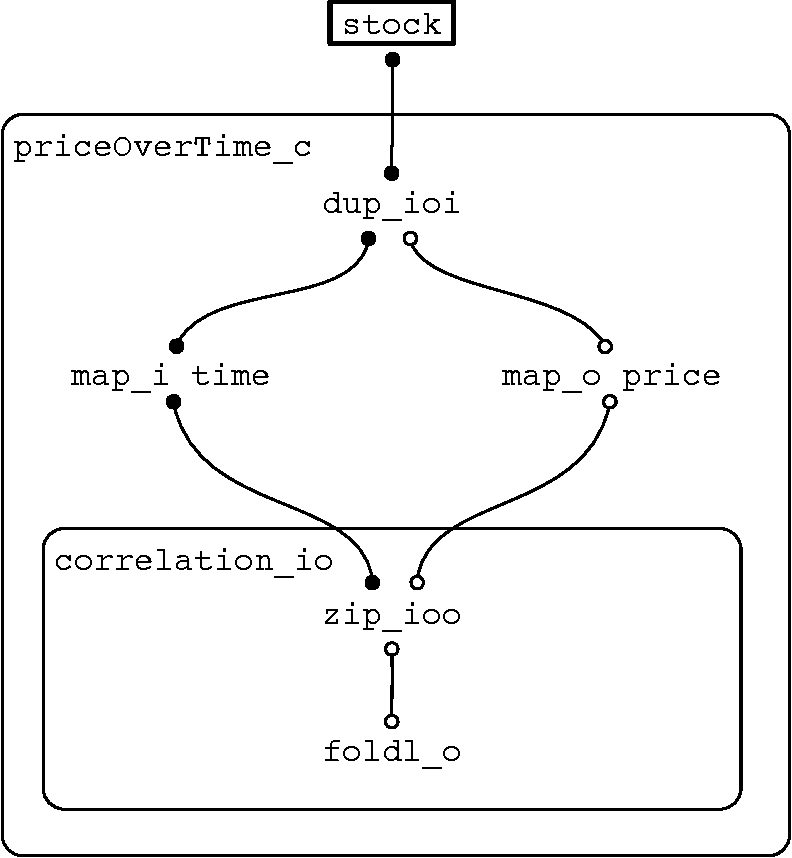
\includegraphics[scale=0.7]{figs/depgraphs/priceOverTime-diamond.pdf}
% \caption{Polarised dependency graph with diamond}
% \label{figs/polar/correlation-zip}
% \end{subfigure}
% \begin{subfigure}[t]{0.4\textwidth}
% 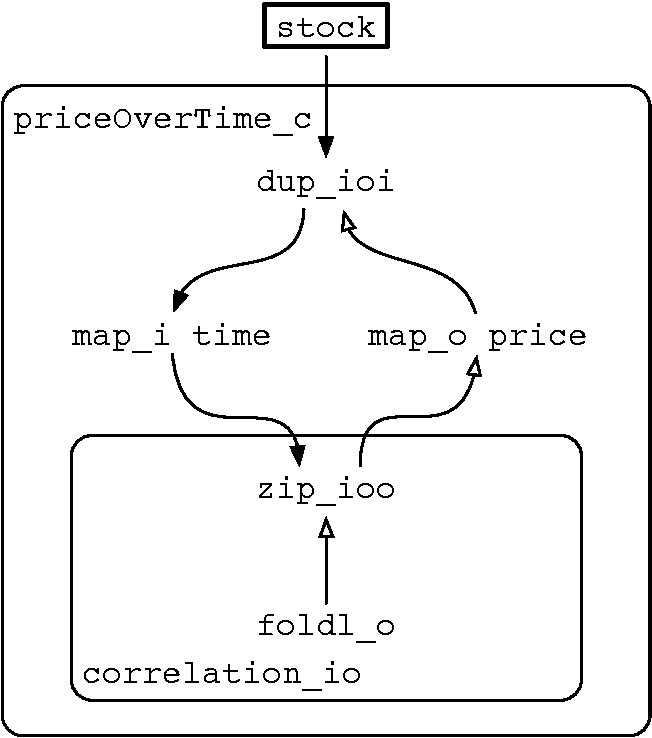
\includegraphics[scale=0.7]{figs/depgraphs/priceOverTime-diamond-cycle.pdf}
% \caption{Control flow graph for polarised diamond}
% \label{figs/control/correlation-zip}
% \end{subfigure}
% \caption{Diamond}
% \label{figs/xxx}
% \end{figure}

\begin{haskell}[float,caption=Polarised implementation of \Hs/zip\_ioo/,label=figs/polar/impl/zip_ioo]
zip_ioo :: PullResult a r -> Push (a,b) r' -> Push b (r,r')
zip_ioo (Pull pull_a) push_ab = Push push_b done_b
 where
  push_b b = do
   a <- pull_a
   case a of
    Left a' -> push push_ab (a',b)
    Right _ -> return ()
  done_b = do
   a <- pull_a
   case a of
    Left _  -> done_b
    Right r -> do
     r' <- done push_ab
     return (r,r')
\end{haskell}


With polarised streams, we cannot execute \Hs@priceOverTime@ with the pair-of-lists version, although we can assign polarities.
The lefthand side of \cref{figs/polar/correlation-zip} shows the polarised graph for a hypothetical version of \Hs@priceOverTime@ that only computes the correlation and uses zip.
The \Hs@zip_ioo@ combinator, implemented in \cref{figs/polar/impl/zip_ioo}, is similar to the \Hs@join_ioo@ combinator; it has an input pull, an input push, and an output push.
When the input push stream receives a value, \Hs@zip_ioo@ reads from the pull stream and sends the pair to the output push stream.


Although it is not obvious from the polarised dependency graph, the combinators have a recursive dependency on each other.
The polarised diagram shows \emph{elements} flowing down, but the \emph{control flow} for push streams is upwards.
The righthand side of \cref{figs/polar/correlation-zip} shows the control flow for the polarised diagram, after replacing the edges corresponding to pull streams with filled downward arrows and replacing the edges corresponding to push streams with unfilled upward arrows.
In this graph, the recursive dependency is illustrated by the cycle between \Hs@dup_ioi@, \Hs@zip_ioo@ and the two maps.
This cycle complicates translating the graph to an implementation.

\begin{haskell}[float,caption={Incomplete polarised implementation of \Hs/priceOverTime_c/},label=figs/polar/impl/priceOverTime_c]
priceOverTime_c :: PullResult Record r -> IO (Double, r)
priceOverTime_c stock =
  let stock' :: PullResult Record (Double,r)
              = dup_ioi stock prices
      times  :: PullResult Record (Double,r)
              = map_i time stock'
      prices :: Push Record Double
              = map_o price cor
      cor    :: Push Record Double
              = correlation_io times
  in _ -- incomplete: no way to run computation

correlation_io :: PullResult Double r -> Push Double (Double, r)
correlation_io stream_a = zip_ioo stream_a correlation_o
\end{haskell}

The incomplete implementation in \cref{figs/polar/impl/priceOverTime_c} also demonstrates the recursive dependency between the four operators.
The \Hs@priceOverTime_c@ function defines a set of stream transformers, but we have no way to execute this stream transformer and extract the result.
The incomplete implementation constructs a stream transformer, but does not directly compute the stream result.
All the combinators are \emph{passive combinators}, constructing a stream transformer that responds to push or pull requests rather than actively pulling or pushing.
\emph{Active combinators} like \Hs/drain_io/ and \Hs/foldl_i/ actively consume pull streams rather than transforming them, and return an \Hs/IO/ action containing the stream result.
Without an active combinator, the query will not execute.
Active combinators can consume pull streams and output to push streams.
Active combinators cannot actively consume push streams, because the control flow for push streams is driven by the producer.
Similarly, they cannot actively produce pull streams.
None of the combinators in this query can be implemented as active combinators because they all consume push streams or produce pull streams.
Instead we must hand-optimise the program, combining the duplicate, maps and zip into one combinator, as in the original version of \Hs@priceOverTime@.


% 
% 
% 
% \subsection{Polarised streams}
% 
% \section{Other streams}
% \subsection{Stream fusion}
% \subsection{Copull: push as pull}
% \subsection{Push-pull, or enumerator}
% \subsection{Monadic streams}
% 

\section{Kahn process networks}
\label{taxonomy/kpn}

The three streaming models we have seen --- pull, push, and polarised streams --- differ essentially in what drives the computation.
With pull streams, the consumer drives the computation.
With push streams, the producer drives the computation.
With polarised streams, the active combinator --- which may be a pull consumer, a push producer, or even both --- drives the computation.
All these systems have one operator driving the computation.
When we have multiple queries to execute, it can be hard to choose just one combinator to drive the entire computation.

An alternate streaming model, which allows many operators to control the computation and supports executing multiple queries, is a \emph{Kahn process network}.
A Kahn process network is a concurrent process network with restrictions to ensure deterministic execution.
Each combinator inside each query becomes a communicating process in the network.
Processes communicate through input channels from which they can pull values, and output channels to which they can push values.
Each process can have multiple inputs and outputs, and the process chooses the order to pull from its inputs and push to its outputs.

Concurrent programs can be hard to write and debug because the \emph{schedule}, which specifies the interleaving of process execution, depends on environmental factors outside the program itself --- for example, the number of physical processors available, and which other processes are also being executed.
Because the environment is not controlled by the processes themselves, we say the schedule is chosen \emph{non-deterministically}.
Likewise, if a program gives different results for different schedules, we say the result is \emph{non-deterministic}.
Kahn process networks are a restricted form of static process network where program values cannot be affected by the schedule \cite{kahn1976coroutines}: the schedule may be chosen non-deterministically, but the result is still deterministic.
Kahn process networks ensure deterministic results by imposing restrictions on how processes communicate so that scheduling decisions cannot be observed inside the process.
% The restrictions are: all communication between processes is through first-in-first-out channels; reading from channels is blocking; and channels are written to by a single process, broadcasting each value to all consumers of the channel.
All communication between processes is through first-in-first-out channels.
The Kahn process network model specifically rules out processes with shared mutable state, as such a process could non-deterministically compute different results.
If one process were reading from mutable state while another were writing a new value, then the reading process may get the old value or new value, depending on how the processes were scheduled.
Reading from channels is blocking: processes cannot to \emph{peek} at a channel to see whether there are waiting values, because another process might be waiting to be scheduled and about to push a new value.
Channels are written to by a single process, broadcasting each value to all consumers of the channel.
Only one process is ever allowed to push to a given channel: if two processes were able to push to the same channel at the same time, the scheduler would have to decide the order in which values were received.

With Kahn process networks, we can implement a process which joins sorted streams by pulling from each input channel as in the \Hs@join@ combinator, and we can share streams among multiple consumers because pushed values are broadcast to each consumer.
We can convert operators that use both push streams and pull streams to processes.
We can also implement a process that copies values from a pull stream into a channel, and a process that copies values from a channel into a push stream.

One version of the Kahn process network model uses bounded channels to ensure that the entire network executes in bounded memory.
Kahn process networks with bounded channels still compute results deterministically, but can introduce \emph{artificial deadlocks} in cases where the computation would succeed with a sufficiently large buffer, but the given bounds are too small.
There are dynamic algorithms to identify artificial deadlocks at runtime and resolve them by increasing buffer sizes \cite{parks1995bounded,geilen2003requirements}.


\begin{haskell}[float,caption=Types and combinators for Kahn process networks,label=figs/kpn/combinators]
data Channel a

data Network a
instance Monad Network

data Result  a
instance Applicative Result

map     :: (a -> b) -> Channel a
        -> Network (Channel b)
join    :: (a -> b -> Ordering) -> Channel a -> Channel b
        -> Network (Channel (a,b))
foldl   :: (a -> b -> a) -> a -> Channel b
        -> Network (Result a)

execute :: Network (Result a) -> IO a
\end{haskell}

\Cref{figs/kpn/combinators} shows the datatypes and type signatures of a Kahn process network implementation.
We leave discussion of the implementation for \cref{chapter:process:processes}, and for now focus solely on this simplified version of the interface.
The \Hs@Channel@ type denotes a communication channel between processes.
The \Hs@Network@ monad describes how to construct a process network; execution is deferred until after the entire network has been constructed.
The \Hs@map@ and \Hs@join@ combinators have type signatures similar to the list versions, with lists replaced by \Hs@Channel@s and the return value inside the \Hs@Network@ monad.

Because execution is deferred, the \Hs@foldl@ combinator cannot return the fold result immediately, and the result is wrapped in a \Hs@Result@ type.
The \Hs@Result@ type describes the result of executing a process network: it is a promise that the value will be available after all the processes in the network finish.
The \Hs@Result@ has an applicative functor instance, allowing multiple results to be combined together.
The \Hs@execute@ function takes a process network description containing the result promise, and executes the processes before extracting the result.



\begin{haskell}[float,caption=Implementation of \Hs/priceAnalyses/ queries as a Kahn process network,label=figs/kpn/impl/priceAnalyses]
correlation :: Channel (Double,Double) -> Network (Result Double)
regression  :: Channel (Double,Double) -> Network (Result Line)

priceOverTime :: Channel Record -> Network (Result (Line,Double)
priceOverTime stock = do
  timeprices <- map (\r -> (daysSinceEpoch (time r), price r)) stock
  r          <- regression  timeprices
  c          <- correlation timeprices
  return ((,) <$> r <*> c)

priceOverMarket :: Channel Record -> Channel Record -> Network (Result (Line,Double))
priceOverMarket stock index = do
  joined <- join (\s i   -> compare (time s) (time i)) stock index
  prices <- map  (\(s,i) -> (price s, price i))        joined
  r      <- regression  prices
  c      <- correlation prices
  return ((,) <$> r <*> c)

priceAnalyses :: Channel Record -> Channel Record
              -> Network (Result ((Line,Double),(Line,Double)))
priceAnalysis stock index = do
  pot <- priceOverTime   stock
  pom <- priceOverMarket stock index
  return ((,) <$> pot <*> pom)
\end{haskell}

\Cref{figs/kpn/impl/priceAnalyses} shows the \Hs@priceAnalyses@ queries implemented as a Kahn process network.
There are some differences from the list version: the process network is constructed inside the \Hs@Network@ monad and the results are paired together using \Hs@Result@ applicative functor instance.
Converting the implementation from the list form to the process network form is almost purely syntactic, in contrast to the polarity analysis required for polarised streams.

Concurrent process networks have the desired high-level semantics for executing concurrent queries, but they do not provide the ideal execution strategy.
In \cref{taxonomy/pull/streaming-overhead}, we saw that communication between pull stream combinators involves allocating \Hs@Maybe@ values, which can sometimes be removed by general purpose compiler optimisations (and sometimes not).
Communication between processes requires more overhead than allocating \Hs@Maybe@ values, and is not removed by general purpose optimisations.
To send a value from one process to another, the sending process may need to lock the communication channel to ensure that it has exclusive access to the channel, before copying the value into a buffer where it can be read by the other process.
Concurrent process network implementations amortise the cost of communication by \emph{chunking} messages together: instead of sending many messages with one value in each, chunked communication sends one message containing an array of values.
Chunking reduces the cost of sending messages, but increases memory and cache pressure.
Chunk size determines how many communications are saved, so larger chunks mean less communication overhead.
However, larger chunks also mean that each chunk array requires more memory and is thus less likely to fit in cache.
Since each channel between a pair of processes requires its own chunk, larger process networks have more chunks in memory at the same time.
The optimal chunk size is a trade-off between communication overhead and memory usage, which is usually found by experimentation.


% consider when one process sends a machine integer to another process.
% If the sending process has performed any computation on the integer, the sending process most likely has the integer stored in a register, where it can be operated on directly by the processor.
% To send this value to the other process, the sending process locks the channel to prevent other writers or premature reads, copies the integer to memory where it can be read by the other process, and unlocks the channel.
% Next, the receiving process performs the inverse operation, locking the channel, copying the integer from memory to a register, and unlocking the channel.
% Sending messages is an expensive way to copy an integer from one register to another register --- perhaps even the same register, if the sending process has been swapped out and the receiving process swapped in.

% Concurrent process network implementations often amortise the cost of communication by \emph{chunking} messages together: instead of sending many messages with an integer in each, chunked communication sends one message containing an array of integers.
% Chunking reduces the cost of sending messages, but cannot eliminate it altogether.
% Chunk size determines how many communications are saved, so larger chunks mean less communication overhead.
% However, larger chunks also mean that each array requires more memory and are less likely to fit in memory or cache.
% Since each channel between processes requires its own chunk, larger process networks tend to have more chunks in memory at the same time.
% Finding the optimal chunk size is a trade-off between communication overhead and memory usage, and finding this optimum usually requires experimentation, with no guarantee that we will be able to find it.

From a functional programming perspective, small, fine-grained processes like those used in our \Hs/priceAnalysis/ example are desirable because they allow us to write a process to implement each combinator and compose them together.
From an execution perspective, however, when fine-grained processes perform more communication than computational work, the overall performance is dominated by synchronisation and scheduling overheads~\cite{chen1990impact}.
We can reduce the amount of communication by fusing multiple connected processes together into one larger process.
The fused process performs the task of multiple individual processes, but communicates by local variables instead of channels.
In \cref{chapter:process:processes} we describe an algorithm to fuse processes together to reduce overhead.
For \Hs@priceAnalysis@, our algorithm can automatically fuse all the processes together into a single processes.
A single process executes sequentially, so fusing the entire network into a single process removes any potential speedup from task parallelism, but in our benchmarks in \cref{s:Benchmarks}, the sequential version is faster than the concurrent version even with several processors.
Often, a well-optimised sequential implementation of a program will consume significantly less power and cost less to run than a parallel implementation~\cite{mcsherry2015scalability}.

% \cite{chen1990impact}
% "We find that even though there can be a lot of parallelism at the fine grain level, synchronization and scheduling strategies determine the ultimate performance of the system."
% "The most important characteristic is that, without the near-optimal scheme, performance at the operation level and at the statement level is actually worse than at the loop-iteration level."
% "unless we have a very sophisticated scheduling strategy, exploiting very fine grain parallelism with only a limited amount of resources can yield poorer results than we have anticipated"

% In \cite{vrba2009evaluating} it ... too much parallelism and not enough work.

% Too much parallelism might make the program \emph{scalable}, in that adding more processors will speed the program, but unfortunately it does not ensure absolute performance.
% In fact, the contrary is often true.
% \cite{mcsherry2015scalability} stresses the importance of measuring against a well-optimised single-threaded implementation when absolute performance is the goal.


\section{Summary}
We have seen the relative advantages of various streaming models.
Pull streams support operators with multiple inputs, and can take advantage of an optimising compiler to reduce overhead.
Push streams support multiple concurrent queries, and are written back-to-front with explicit duplication for sharing streams.
Polarised streams support multiple inputs and multiple queries, require polarity analysis of the entire dependency graph, and are written partially back-to-front and partially front-to-back.
Kahn process networks support multiple inputs and multiple queries, and concurrent execution involves communication overhead.

In the next chapter we will see Icicle, a language for specifying push stream queries.
Icicle queries are written front-to-back, and streams can be shared without requiring explicit duplication.
Queries are compiled to folds over push streams which can be executed concurrently.
After looking at Icicle, we shall see how Kahn process networks can be executed efficiently by fusing processes together (\cref{chapter:process:processes}).

